
\section{Paragraf autorstwa Mateusza Porębskiego}

Znane jest każdemu równianie autorstwa Alberta Einsteina:
    \begin{equation} \label{eq:1}
        e = mc^2 
    \end{equation}
    Tak samo jak i wzór Pitagorasa nikomu raczej nie musi być przypominany:
    \begin{equation} \label{eq:2}
        c^2 = a^2 + b^2
    \end{equation} 
    Możemy zatem podstawić do wzoru (\ref{eq:1}) $c^2$ ze wzoru (\ref{eq:2}). Dostajemy wtedy:

    \begin{equation} \label{eq:3}
        e = m(a^2 + b^2)
    \end{equation}
    \begin{equation} \label{eq:4}
        e = ma^2 + mb^2
    \end{equation}
    Dane przekrztałcenie jest przydatne gdy chcemy obliczyć \textbf{energię} ciała o danej \textbf{masie} i \textbf{długościach przekątych}, \underline{a akurat nie pamiętamy prędkości światła}.
    \begin{figure}[htbp]
        \centering
        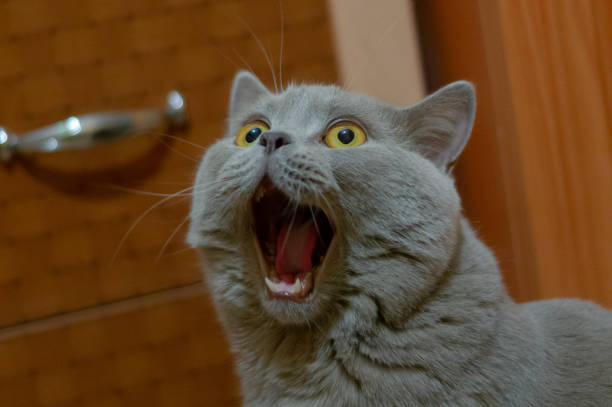
\includegraphics[width=0.5\textwidth]{pictures/heckin_cute.jpg}
        \caption{He's absolutely amazed}
        \label{fig:hecingcute}
    \end{figure}


Jak widać na Rysunku~\ref{fig:hecingcute} on jest absolutnie zachwycony

\begin{table}[htbp]
\centering
\begin{tabular}{|
>{\columncolor[HTML]{FFCE93}}l |l|l|l|l}
\cline{1-4}
\cellcolor[HTML]{F8A102}{\color[HTML]{333333} \textbf{wyniki}} & \cellcolor[HTML]{F8A102}{\color[HTML]{333333} \textbf{''Maciek''}} & \cellcolor[HTML]{F8A102}{\color[HTML]{333333} \textbf{''Anna''}} & \cellcolor[HTML]{F8A102}{\color[HTML]{333333} \textbf{''Jaś''}} &  \\ \cline{1-4}
\textit{styczeń}                                               & 12                                                             & 123                                                          & 551                                                         &  \\ \cline{1-4}
\textit{luty}                                                  & 231                                                            & 412                                                          & 2212                                                        &  \\ \cline{1-4}
\textit{marzec}                                                & 33                                                             & 3311                                                         & 21                                                          &  \\ \cline{1-4}
\end{tabular}
\label{tab:osoby}
\caption{Wyniki poszczególnych ''osób'' w poszczególnych miesiącach}
\end{table}
Tak samo tutaj (Tabela~\ref{tab:osoby}) widać wyniki poszczególnych ''osób'' w poszczególnych miesiącach

\subsection{Listy nienumerowane i numerowane}

Lista nienumerowana:
\begin{itemize} \label{nienumerowana}
  \item Pierwszy element
  \item Drugi element
  \item Czwarty element
\end{itemize}

Lista numerowana
\begin{enumerate}
    \item numeracja 
    \item działa
    \item automatycznie
\end{enumerate}
